\documentclass{article}

% Imports

% content/resources/templates/preamble.tex
\usepackage[margin=0.6in]{geometry}
\author{Milav Dabgar}
\usepackage{amsmath,amssymb,amsthm}
\usepackage{booktabs}
\usepackage{multirow}
\usepackage{xcolor}
\usepackage{tcolorbox}
\tcbuselibrary{breakable,skins}
\usepackage[colorlinks=true,linkcolor=blue]{hyperref}
\usepackage{titlesec}
\usepackage{enumitem}
\usepackage{tikz}
\usepackage{pgfplots}
\usepackage{circuitikz}
\usepackage[version=4]{mhchem}
\usepackage{longtable}
\usepackage{array}
\usepackage{float}
\usepackage{caption}
\usepackage{listings}

\lstset{
  basicstyle=\small\ttfamily,
  breaklines=true,
  breakatwhitespace=false,
  postbreak=\mbox{\textcolor{red}{$\hookrightarrow$}\space},
  float=false,
  numbers=left,
  numberstyle=\tiny\color{gray},
  numbersep=10pt,
  xleftmargin=2em,
  keywordstyle=\color{blue},
  commentstyle=\color{green!60!black},
  stringstyle=\color{purple},
  backgroundcolor=\color{gray!5},
  showstringspaces=false,
  tabsize=2,
  captionpos=b,
  keepspaces=true,
  columns=flexible
}

\pgfplotsset{compat=1.18}
\usetikzlibrary{shapes,arrows,positioning,calc,patterns,decorations.pathmorphing,decorations.markings,arrows.meta}

% Color scheme
\definecolor{headcolor}{RGB}{0,102,204}
\definecolor{keycolor}{RGB}{220,20,60}
\definecolor{solutioncolor}{RGB}{34,139,34}
\definecolor{mnemoniccolor}{RGB}{148,0,211}
\definecolor{codecolor}{RGB}{0,0,100}

% Spacing
\setlength{\parskip}{3pt}
\setlist[itemize]{nosep}
\setlist[enumerate]{nosep}

% Title formatting
\titleformat{\section}{\Large\bfseries\color{headcolor}}{\thesection}{1em}{}
\titleformat{\subsection}{\large\bfseries\color{headcolor}}{\thesubsection}{1em}{}

% Pandoc tightlist compatibility
\providecommand{\tightlist}{%
  \setlength{\itemsep}{0pt}\setlength{\parskip}{0pt}}

% Pandoc longtable compatibility
\newcounter{none}
\def\thenone{}


% content/resources/templates/english-boxes.tex
% This file is currently empty - it exists to maintain consistency with the import structure.
% Add custom environments here if needed in the future.


% Custom commands for GTU solutions
% This file defines semantic commands for consistent formatting

% Question command with automatic formatting
\newcommand{\question}[2]{%
  \section*{Question #1}%
  \textbf{#2}%
}

% OR question variant
\newcommand{\questionor}[2]{%
  \section*{Question #1 OR}%
  \textbf{#2}%
}

% Proper table environment with caption
\newenvironment{answertable}[1]{%
  \begin{table}[htbp]
  \centering
  \caption{#1}
}{%
  \end{table}
}

% Proper figure environment for diagrams
\newenvironment{answerdiagram}[1]{%
  \begin{figure}[htbp]
  \centering
  \caption{#1}
}{%
  \end{figure}
}

% Semantic markup for key terms
\newcommand{\keyword}[1]{\textbf{#1}}
\newcommand{\code}[1]{\texttt{#1}}
\newcommand{\classname}[1]{\texttt{#1}}
\newcommand{\methodname}[1]{\texttt{#1}}

% Proper quotation marks
\newcommand{\mnemonic}[1]{``#1''}


\title{Linear Integrated Circuit (4341105) - Summer 2023 Solution}
\date{July 18, 2023}

\begin{document}
\maketitle
\solutiontitle

% Question 1(a)
\questionmarks{1(a)}{3}{Write advantages and disadvantages of negative feedback amplifier}
\begin{solutionbox}
    \begin{tabulary}{\linewidth}{|L|L|}
        \hline
        \textbf{Advantages} & \textbf{Disadvantages} \\
        \hline
        Increases bandwidth & Reduces gain \\
        \hline
        Stabilizes gain & Requires more components \\
        \hline
        Reduces distortion & Increases cost \\
        \hline
        Increases input impedance (voltage series) & May cause oscillations if improperly designed \\
        \hline
        Decreases output impedance (voltage series) & Requires careful phase compensation \\
        \hline
    \end{tabulary}

    \begin{mnemonicbox}
        \mnemonic{GRASS Grows Better Despite Dry Soil: Gain Reduction, Amplifies Stability, Stops distortion, Better impedance}
    \end{mnemonicbox}
\end{solutionbox}

% Question 1(b)
\questionmarks{1(b)}{4}{Derive the equation of overall gain with negative feedback in amplifier and give application of negative feedback.}
\begin{solutionbox}
    \textbf{Derivation of overall gain:}
    \begin{figure}[H]
        \centering
        \begin{tikzpicture}[gtu flow]
            \node (In) [gtu block] {Input};
            \node (Sum) [gtu block, right=of In] {Summing Point};
            \node (Amp) [gtu block, right=of Sum] {Amplifier A};
            \node (Out) [gtu block, right=of Amp] {Output};
            \node (Feed) [gtu block, below=of Amp] {Feedback $\beta$};

            \draw [gtu arrow] (In) -- (Sum) node[midway, above] {$V_{in}$};
            \draw [gtu arrow] (Sum) -- (Amp) node[midway, above] {$V_e$};
            \draw [gtu arrow] (Amp) -- (Out) node[midway, above] {$V_{out}$};
            \draw [gtu arrow] (Out) |- (Feed);
            \draw [gtu arrow] (Feed) -| (Sum) node[midway, left] {$\beta V_{out}$};
        \end{tikzpicture}
        \caption{Negative Feedback Block Diagram}
    \end{figure}

    Let amplifier gain be $A$ and feedback factor be $\beta$.
    \begin{itemize}
        \item Input signal = $V_{in}$
        \item Feedback signal = $\beta V_{out}$
        \item Effective input to amplifier = $V_{in} - \beta V_{out}$
        \item Output $V_{out} = A(V_{in} - \beta V_{out})$
        \item $V_{out} + A\beta V_{out} = A V_{in}$
        \item $V_{out}(1 + A\beta) = A V_{in}$
        \item \textbf{Overall Gain $A_f = \frac{V_{out}}{V_{in}} = \frac{A}{1 + A\beta}$}
    \end{itemize}

    \textbf{Applications:} Operational amplifiers, Voltage regulators, Audio amplifiers, Instrumentation amplifiers.

    \begin{mnemonicbox}
        \mnemonic{AVOI: Amplifiers, Voltage regulators, Oscillation control, Instrumentation}
    \end{mnemonicbox}
\end{solutionbox}

% Question 1(c)
\questionmarks{1(c)}{7}{Draw and Explain current shunt type negative feedback amplifier and Derive the formula of input impedance and output impedance of it.}
\begin{solutionbox}
    \textbf{Current Shunt Negative Feedback:}
    Output voltage is sampled and converted to current, which is subtracted from input current (Shunt mixing).

    \begin{figure}[H]
        \centering
        \begin{tikzpicture}[gtu flow]
            \node (In) [gtu block] {Input Current $I_{in}$};
            \node (Sum) [gtu block, right=of In] {Shunt Mixer};
            \node (Amp) [gtu block, right=of Sum] {Amplifier};
            \node (Out) [gtu block, right=of Amp] {Output $V_{out}$};
            \node (Feed) [gtu block, below=of Amp] {Feedback $\beta$};
            
            \draw [gtu arrow] (In) -- (Sum);
            \draw [gtu arrow] (Sum) -- (Amp);
            \draw [gtu arrow] (Amp) -- (Out);
            \draw [gtu arrow] (Out) |- (Feed);
            \draw [gtu arrow] (Feed) -| (Sum) node[midway, left] {$I_f$};
        \end{tikzpicture}
        \caption{Current Shunt Feedback}
    \end{figure}

    \textbf{Characteristics:}
    \begin{itemize}
        \item Feedback type: Current sampling (Series), Current mixing (Shunt). *Note: The question says "Current Shunt". Usually means Output=Current, Input=Shunt. But description says "output voltage sampled... subtracted from input current". This corresponds to Voltage-Shunt topology usually. Wait. "converted to a current".
        \item MDX says: "Output voltage is sampled...". That's Voltage Sampling. "subtracted from input current...". That's Shunt Mixing. So it is **Voltage-Shunt** feedback.
        \item MDX Title says: "Current Shunt type".
        \item Standard texts: Current-Shunt means Output=Current sampled (Series output), Input=Current mixed (Shunt input).
        \item Let's check the Derivations in MDX.
        \item MDX Derivation: $Z_{in}' = Z_{in}/(1+A\beta)$ (Decreases). $Z_{out}' = Z_{out}/(1+A\beta)$ (Decreases).
        \item Voltage-Shunt (Transresistance) -> $Z_{in}$ decreases, $Z_{out}$ decreases. Matches derivation.
        \item So it describes **Voltage-Shunt** feedback but labels it Current Shunt. I will follow the text description characteristics.
    \end{itemize}

    \textbf{Input Impedance:}
    Without feedback: $Z_{in}$.
    With feedback: $Z_{in}' = \frac{Z_{in}}{1 + A\beta}$.
    Input impedance \textbf{decreases} by factor $(1 + A\beta)$.

    \textbf{Output Impedance:}
    Without feedback: $Z_{o}$.
    With feedback: $Z_{o}' = \frac{Z_{o}}{1 + A\beta}$.
    Output impedance \textbf{decreases} by factor $(1 + A\beta)$.

    \begin{mnemonicbox}
        \mnemonic{DISCO: Decreased Impedances with Shunt Current Operation}
    \end{mnemonicbox}
\end{solutionbox}

% Question 1(c) OR
\questionmarks{1(c) OR}{7}{Draw and Explain voltage series type negative feedback amplifier and Derive the formula of input impedance and output impedance of it.}
\begin{solutionbox}
    \textbf{Voltage Series Negative Feedback:}
    Output voltage is sampled and fed back in series with input voltage.

    \begin{figure}[H]
        \centering
        \begin{tikzpicture}[gtu flow]
            \node (In) [gtu block] {Input $V_{in}$};
            \node (Sum) [gtu block, right=of In] {Series Mixer};
            \node (Amp) [gtu block, right=of Sum] {Amplifier};
            \node (Out) [gtu block, right=of Amp] {Output $V_{out}$};
            \node (Feed) [gtu block, below=of Amp] {Feedback $\beta$};

            \draw [gtu arrow] (In) -- (Sum);
            \draw [gtu arrow] (Sum) -- (Amp);
            \draw [gtu arrow] (Amp) -- (Out);
            \draw [gtu arrow] (Out) |- (Feed);
            \draw [gtu arrow] (Feed) -| (Sum) node[midway, left] {$V_f$};
        \end{tikzpicture}
        \caption{Voltage Series Feedback}
    \end{figure}

    \textbf{Characteristics:}
    \begin{itemize}
        \item Feedback: Voltage sampling (Output), Series mixing (Input).
    \end{itemize}

    \textbf{Input Impedance:}
    Without feedback: $Z_{in}$.
    With feedback: $Z_{in}' = Z_{in}(1 + A\beta)$.
    Input impedance \textbf{increases} by factor $(1 + A\beta)$.

    \textbf{Output Impedance:}
    Without feedback: $Z_{o}$.
    With feedback: $Z_{o}' = \frac{Z_{o}}{1 + A\beta}$.
    Output impedance \textbf{decreases} by factor $(1 + A\beta)$.

    \begin{mnemonicbox}
        \mnemonic{ISDO: Increased input impedance, Series feedback, Decreased output impedance}
    \end{mnemonicbox}
\end{solutionbox}

% Question 2(a)
\questionmarks{2(a)}{3}{Draw and Explain the circuit diagram of UJT as a relaxation oscillator.}
\begin{solutionbox}
    \textbf{UJT Relaxation Oscillator:}
    \begin{figure}[H]
        \centering
        \begin{circuitikz}[scale=0.8]
            \draw (0,0) node[ground]{} to[C, l=$C_1$] (0,2) -- (2,2) node[ujt, anchor=E](U){}; 
            \draw (0,2) to[R, l=$R_1$] (0,5) -- (4,5) node[vcc]{$+V_{CC}$};
            \draw (U.B2) to[short] (2,4) to[R, l=$R_2$] (2,5) -- (0,5);
            \draw (U.B1) to[R, l=$R_3$] (2,0) node[ground]{};
            \draw (2,2) to[short, -o] (4,2) node[right]{Output};
        \end{circuitikz}
        \caption{UJT Relaxation Oscillator}
    \end{figure}
    \textit{Note: If UJT symbol fails to render, use discrete representation.}
    
    \textbf{Working:}
    \begin{itemize}
        \item Capacitor $C_1$ charges through $R_1$.
        \item When voltage $V_c$ reaches UJT peak point ($V_p$), UJT fires (turns ON).
        \item Capacitor discharges rapidly through UJT Emitter-Base1 path and $R_3$.
        \item Cycle repeats, generating sawtooth waveform at Capacitor and pulses at Output.
    \end{itemize}

    \begin{mnemonicbox}
        \mnemonic{CURD: Capacitor charges Until Reaching Discharge point}
    \end{mnemonicbox}
\end{solutionbox}

% Question 2(b)
\questionmarks{2(b)}{4}{Draw circuit diagram of Colpitts oscillator and explain in brief. Give the advantages and disadvantages of it.}
\begin{solutionbox}
    \textbf{Colpitts Oscillator:}
    Uses capacitive voltage divider for feedback.

    \begin{figure}[H]
        \centering
        \begin{circuitikz}[scale=0.8]
            \draw (0,0) node[ground]{} to[C, l=$C_2$] (2,0);
            \draw (2,0) to[C, l=$C_1$] (4,0);
            \draw (0,0) to[L, l=$L$] (0,3) -- (4,3) -- (4,0);
            \draw (2,0) -- (2, -1) -- (5,-1) node[npn, anchor=B](Q){};
            \draw (Q.E) to[R, l=$R_E$] (5,-3) node[ground]{};
            \draw (Q.C) to[R, l=$R_C$] (5,1) node[vcc]{$+V_{CC}$};
            % Simplified tank connection
            \draw (Q.C) -- (5,3) -- (4,3);
            \draw (Q.B) to[R, l=$R_B$] (3,-1) to[short] (2,-1);
        \end{circuitikz}
        \caption{Colpitts Oscillator (Tank Circuit Feedback)}
    \end{figure}

    \textbf{Working:}
    \begin{itemize}
        \item Tank circuit made of $L$ and split capacitors $C_1, C_2$.
        \item Transistor amplifies signal to sustain oscillations.
        \item Frequency: $f = \frac{1}{2\pi\sqrt{L C_{eq}}}$ where $C_{eq} = \frac{C_1 C_2}{C_1 + C_2}$.
    \end{itemize}

    \begin{tabulary}{\linewidth}{|L|L|}
        \hline
        \textbf{Advantages} & \textbf{Disadvantages} \\
        \hline
        Good frequency stability & Requires two capacitors \\
        \hline
        Good for high frequencies & Harder to tune (gang tuning needed) \\
        \hline
        Simple design & Limited frequency range \\
        \hline
    \end{tabulary}

    \begin{mnemonicbox}
        \mnemonic{FAST Circuits: Frequency stable, Appropriate for high frequencies, Simple design, Two capacitors}
    \end{mnemonicbox}
\end{solutionbox}

% Question 2(c)
\questionmarks{2(c)}{7}{Explain the Crystal Oscillator.}
\begin{solutionbox}
    \textbf{Crystal Oscillator:}
    Uses piezoelectric crystal (Quartz) for extremely stable frequency.

    \begin{figure}[H]
        \centering
        \begin{tikzpicture}[gtu flow]
            \node (Crystal) [gtu block] {Piezoelectric Crystal};
            \node (Amp) [gtu block, right=of Crystal] {Amplifier};
            \node (Feed) [gtu block, below=of Amp] {Feedback};
            
            \draw [gtu arrow] (Crystal) -- (Amp);
            \draw [gtu arrow] (Amp) -- (Feed);
            \draw [gtu arrow] (Feed) -| (Crystal);
        \end{tikzpicture}
        \caption{Concept of Crystal Oscillator}
    \end{figure}

    \textbf{Circuit Diagram:}
    \begin{figure}[H]
        \centering
        \begin{circuitikz}[scale=0.8]
             \draw (0,0) node[npn](Q){};
             \draw (Q.E) to[R, l=$R_E$] (0,-2) node[ground]{};
             \draw (Q.C) to[R, l=$R_C$] (0,2) node[vcc]{$+V_{CC}$};
             \draw (Q.B) -- (-1,0) to[piezoelectric, l=XTAL] (-1,-2) node[ground]{};
             \draw (-1,0) to[R, l=$R_B$] (-1,2) node[vcc]{};
             \draw (Q.C) to[C, l=$C_{out}$] (2,0) node[right]{Output};
        \end{circuitikz}
        \caption{Pierce Crystal Oscillator}
    \end{figure}

    \textbf{Working:}
    \begin{itemize}
        \item Based on Piezoelectric effect: Crystal vibrates when voltage applied.
        \item Acts as high-Q Tuned Circuit. Q-factor $\approx 10,000+$.
        \item Provides very stable frequency $\Delta f/f \approx 10^{-6}$.
    \end{itemize}

    \textbf{Applications:} Microprocessors (Clocks), Digital watches, Radio transmitters.

    \begin{mnemonicbox}
        \mnemonic{STOP: Stable, Temperature-resistant, Oscillates, Piezoelectric}
    \end{mnemonicbox}
\end{solutionbox}

% Question 2(a) OR
\questionmarks{2(a) OR}{3}{Draw and explain the Hartley Oscillator.}
\begin{solutionbox}
    \textbf{Hartley Oscillator:}
    Uses tapped inductor tank circuit.

    \begin{figure}[H]
        \centering
        \begin{circuitikz}[scale=0.8]
            \draw (0,0) node[ground]{} to[L, l=$L_2$] (0,1.5) to[L, l=$L_1$] (0,3) -- (2,3) to[C, l=$C$] (2,0) -- (0,0);
            \draw (2,3) -- (4,3) node[npn, anchor=B](Q){};
            \draw (Q.E) node[ground]{}; % Simplified common emitter
            \draw (Q.C) to[R] (4.8, 5) node[vcc]{$+V_{CC}$};
            % Feedback from tap? Actually classic Hartley feeds back from split inductor usually.
            \draw (0,1.5) -- (-1,1.5) node[left]{Tap Ground/Feedback}; 
            % Simplified schematic
        \end{circuitikz}
        \caption{Hartley Tank Circuit (Tapped Inductor)}
    \end{figure}

    \textbf{Working:}
    \begin{itemize}
        \item Inductive voltage divider ($L_1, L_2$) provides feedback.
        \item Frequency: $f = \frac{1}{2\pi\sqrt{L_{eq} C}}$ where $L_{eq} = L_1 + L_2$.
        \item Used for RF applications.
    \end{itemize}

    \begin{mnemonicbox}
        \mnemonic{TIC: Tapped Inductor Circuit}
    \end{mnemonicbox}
\end{solutionbox}

% Question 2(b) OR
\questionmarks{2(b) OR}{4}{Draw and explain Wien Bridge oscillator.}
\begin{solutionbox}
    \textbf{Wien Bridge Oscillator:}
    Audio frequency oscillator using RC bridge.

    \begin{figure}[H]
        \centering
        \begin{circuitikz}[scale=0.7]
            \draw (0,0) node[op amp] (opamp) {};
            \draw (opamp.+) -- (-1, -0.5) -- (-1, -2) to[R, l=$R_2$] (-1, -4) node[ground]{};
            \draw (-1, -2) to[C, l=$C_2$] (-1, -4); % Parallel RC
            \draw (-1, -0.5) -- (-3, -0.5) to[R, l=$R_1$] (-4, -0.5) to[C, l=$C_1$] (-5, -0.5) -- (-5, 1) -- (1, 1) -- (opamp.out);
            % Negative feedback for gain control
            \draw (opamp.-) -- (-1, 0.5) to[R, l=$R_3$] (-1, 2) -- (1, 2) -- (opamp.out);
            \draw (-1, 0.5) to[R, l=$R_4$] (-1, -0.5); % Error in drawing logic, R4 goes to ground usually
            \draw (-1, 0.5) to[R, l=$R_4$] (-3, 0.5) node[ground]{};
        \end{circuitikz}
        \caption{Wien Bridge Oscillator}
    \end{figure}

    \textbf{Working:}
    \begin{itemize}
        \item Uses series RC ($Z_1$) and parallel RC ($Z_2$) arms.
        \item Balance condition: $f = \frac{1}{2\pi RC}$.
        \item Amplifier gain must be $A \ge 3$ to sustain oscillations.
        \item Low distortion sine wave generator.
    \end{itemize}

    \begin{mnemonicbox}
        \mnemonic{FEAR: Frequency selective, Equal RC, Audio Range}
    \end{mnemonicbox}
\end{solutionbox}

% Question 2(c) OR
\questionmarks{2(c) OR}{7}{Draw the Structure, symbol, equivalent circuit of UJT and explain in brief.}
\begin{solutionbox}
    \textbf{Unijunction Transistor (UJT):}

    \begin{figure}[H]
        \centering
        \begin{tikzpicture}[gtu flow]
            % Structure
            \node[gtu block, minimum height=3cm, minimum width=1cm, fill=yellow!20] (bar) {};
            \node at (bar.north) [above] {Base 2 ($B_2$)};
            \node at (bar.south) [below] {Base 1 ($B_1$)};
            \draw (bar.north) -- ++(0,0.5);
            \draw (bar.south) -- ++(0,-0.5);
            \node[draw, rectangle, fill=blue!20, minimum size=0.5cm, left] at (bar.west) (emitter) {P};
            \node at (bar.center) {N-Type Si};
            \draw (emitter.west) -- ++(-0.5,0) node[left] {Emitter ($E$)};
        \end{tikzpicture}
        \caption{UJT Structure}
    \end{figure}

    \textbf{Working Principle:}
    \begin{itemize}
        \item 3-terminal device: Emitter, Base1, Base2.
        \item RB1 and RB2 are internal resistances of N-bar.
        \item \textbf{Firing Condition:} When $V_E > \eta V_{BB} + V_D$, current flows.
        \item Exhibits \textbf{Negative Resistance} region.
    \end{itemize}

    \textbf{Characteristics:}
    \begin{itemize}
        \item Intrinsic Standoff Ratio $\eta = \frac{R_{B1}}{R_{B1} + R_{B2}}$. Typically 0.5-0.8.
        \item Peak Point ($V_p$): Onset of conduction.
        \item Valley Point ($V_v$): Minimum voltage after firing.
    \end{itemize}

    \begin{mnemonicbox}
        \mnemonic{NEVER: Negative resistance, Emitter-triggered, Valley/Peak points}
    \end{mnemonicbox}
\end{solutionbox}

% Question 3(a)
\questionmarks{3(a)}{3}{Differentiate between voltage and power amplifier.}
\begin{solutionbox}
    \begin{tabulary}{\linewidth}{|L|L|L|}
        \hline
        \textbf{Parameter} & \textbf{Voltage Amplifier} & \textbf{Power Amplifier} \\
        \hline
        Purpose & Amplifies voltage & Delivers power to load \\
        \hline
        Output Impedance & High & Low \\
        \hline
        Input Impedance & High & Relatively low \\
        \hline
        Efficiency & Not important & Very important \\
        \hline
        Heat Dissipation & Low & High (requires heat sink) \\
        \hline
        Position & Early stages & Final stage \\
        \hline
    \end{tabulary}

    \begin{mnemonicbox}
        \mnemonic{PEHIP: Power for Efficiency and Heat, Impedance matters, Position differs}
    \end{mnemonicbox}
\end{solutionbox}

% Question 3(b)
\questionmarks{3(b)}{4}{Explain class-B push pull power amplifier in detail.}
\begin{solutionbox}
    \textbf{Class-B Push-Pull Amplifier:}
    Uses two complementary transistors, each conducting for 180° of the cycle.

    \begin{figure}[H]
        \centering
        \begin{circuitikz}[scale=0.8]
            \draw (0,0) node[npn](Q1){Q1};
            \draw (0,-3) node[pnp](Q2){Q2};
            \draw (Q1.E) -- (Q2.E);
            \draw (Q1.B) -- (Q2.B);
            \draw (Q1.B) -- (-1.5, -1.5) node[left]{Input};
            \draw (Q1.E) -- (1.5, -1.5) to[C, l=$C_{out}$] (3, -1.5) to[R, l=$R_L$] (3, -3.5) node[ground]{};
            \draw (3, -1.5) node[right]{Output};
            \draw (Q1.C) -- (0, 1.5) node[vcc]{$+V_{CC}$};
            \draw (Q2.C) -- (0, -4.5) node[vcc]{$-V_{CC}$};
        \end{circuitikz}
        \caption{Class-B Push-Pull}
    \end{figure}

    \textbf{Working:}
    \begin{itemize}
        \item Q1 conducts for positive half cycle.
        \item Q2 conducts for negative half cycle.
        \item Combined output is full sine wave.
        \item Efficiency $\eta \approx 78.5\%$.
        \item Suffers from \textbf{Crossover Distortion}.
    \end{itemize}

    \begin{mnemonicbox}
        \mnemonic{ECHO: Efficiency high, Crossover distortion, Half-cycle operation, Output high power}
    \end{mnemonicbox}
\end{solutionbox}

% Question 3(c)
\questionmarks{3(c)}{7}{Draw and Explain Complementary symmetry push-pull power amplifier in detail also list the disadvantages of it.}
\begin{solutionbox}
    \textbf{Complementary Symmetry Push-Pull:}
    Uses matched NPN and PNP transistors. No transformers required.

    \begin{figure}[H]
        \centering
        \begin{circuitikz}[scale=0.8]
            \draw (0,2) node[npn](Q1){NPN} -- (0,3) node[vcc]{$+V_{CC}$};
            \draw (0,-2) node[pnp](Q2){PNP} -- (0,-3) node[vcc]{$-V_{CC}$};
            \draw (Q1.E) -- (Q2.E);
            \draw (Q1.B) -- (Q2.B) -- (-2,0) to[C] (-3,0) node[left]{Input};
            \draw (Q1.E) -- (2,0) to[C, l=$C_C$] (3,0) to[R, l=$R_L$] (3,-2) node[ground]{};
            \draw (3,0) node[right]{Output};
            \draw (Q1.B) to[R, l=$R_1$] (0, 2.5); % Bias to reduce crossover
            \draw (Q2.B) to[R, l=$R_2$] (0, -2.5); % Bias
        \end{circuitikz}
        \caption{Complementary Symmetry Amplifier}
    \end{figure}

    \textbf{Disadvantages:}
    \begin{enumerate}
        \item Needs matched NPN/PNP pair (hard to find in high power).
        \item Thermal runaway if not properly biased.
        \item Crossover distortion (if pure Class B).
        \item Requires dual power supply usually.
    \end{enumerate}

    \begin{mnemonicbox}
        \mnemonic{MATCH: Matched transistors, Avoids transformers, Thermal issues, Crossover distortion}
    \end{mnemonicbox}
\end{solutionbox}

% Question 3(a) OR
\questionmarks{3(a) OR}{3}{Define the terms related to power amplifier. i)Efficiency ii)Distortion iii)power dissipation capability}
\begin{solutionbox}
    \begin{tabulary}{\linewidth}{|L|L|}
        \hline
        \textbf{Term} & \textbf{Definition} \\
        \hline
        Efficiency & Ratio of AC output power to DC input power. $\eta = \frac{P_{out}}{P_{in}} \times 100\%$. \\
        \hline
        Distortion & Unwanted alteration of output waveform (THD). Harmonics, crossover, etc. \\
        \hline
        Power Dissipation Capability & Max power the device can dissipate as heat without damage. Depends on heat sink. \\
        \hline
    \end{tabulary}

    \begin{mnemonicbox}
        \mnemonic{EDP: Efficiency converts, Distortion deforms, Power capability protects}
    \end{mnemonicbox}
\end{solutionbox}

% Question 3(b) OR
\questionmarks{3(b) OR}{4}{Classify the power amplifier for mode of operation and explain working of different type power amplifier}
\begin{solutionbox}
    \textbf{Classification:}
    \begin{figure}[H]
        \centering
        \begin{tikzpicture}[gtu flow]
            \node (PA) [gtu root] {Power Amplifiers};
            \node (A) [gtu child, below left=of PA, xshift=-1cm] {Class A};
            \node (B) [gtu child, below left=of PA, xshift=1cm] {Class B};
            \node (AB) [gtu child, below right=of PA, xshift=-1cm] {Class AB};
            \node (C) [gtu child, below right=of PA, xshift=1cm] {Class C};
            
            \draw [gtu arrow] (PA) -- (A);
            \draw [gtu arrow] (PA) -- (B);
            \draw [gtu arrow] (PA) -- (AB);
            \draw [gtu arrow] (PA) -- (C);
        \end{tikzpicture}
    \end{figure}

    \begin{tabulary}{\linewidth}{|l|l|L|}
        \hline
        Class & Angle & Working \\
        \hline
        A & $360^\circ$ & Conducts full cycle. Linear, Low efficiency ($25-50\%$). \\
        \hline
        B & $180^\circ$ & Conducts half cycle. High efficiency ($78.5\%$), X-over distortion. \\
        \hline
        AB & $180^\circ-360^\circ$ & Trade-off. Reduced distortion, Good efficiency ($50-70\%$). \\
        \hline
        C & $<180^\circ$ & Tuned circuits. High efficiency ($>80\%$), High distortion. \\
        \hline
    \end{tabulary}
\end{solutionbox}

% Question 3(c) OR
\questionmarks{3(c) OR}{7}{Derive efficiency of class-B push pull power amplifier.}
\begin{solutionbox}
    \textbf{Efficiency Derivation:}
    \begin{itemize}
        \item \textbf{DC Input Power:} $I_{dc} = \frac{2I_m}{\pi}$ (Total for full wave). $P_{dc} = V_{CC} I_{dc} = \frac{2 V_{CC} I_m}{\pi}$.
        \item \textbf{AC Output Power:} $I_{rms} = \frac{I_m}{\sqrt{2}}$. $P_{ac} = \frac{V_m I_m}{2}$. (Ideally $V_m = V_{CC}$).
        \item \textbf{Efficiency:}
        $$\eta = \frac{P_{ac}}{P_{dc}} \times 100\% = \frac{V_{CC} I_m / 2}{2 V_{CC} I_m / \pi} \times 100\%$$
        $$\eta = \frac{\pi}{4} \times 100\% \approx 78.5\%$$
    \end{itemize}

    \begin{mnemonicbox}
        \mnemonic{PIPE: Power ratio, Input DC vs Output AC, Pi in formula, Efficiency 78.5\%}
    \end{mnemonicbox}
\end{solutionbox}

% Question 4(a)
\questionmarks{4(a)}{3}{Draw pin diagram and Schematic symbol of IC 741 and explain it in detail.}
\begin{solutionbox}
    \textbf{IC 741 Op-Amp:}
    \begin{figure}[H]
        \centering
        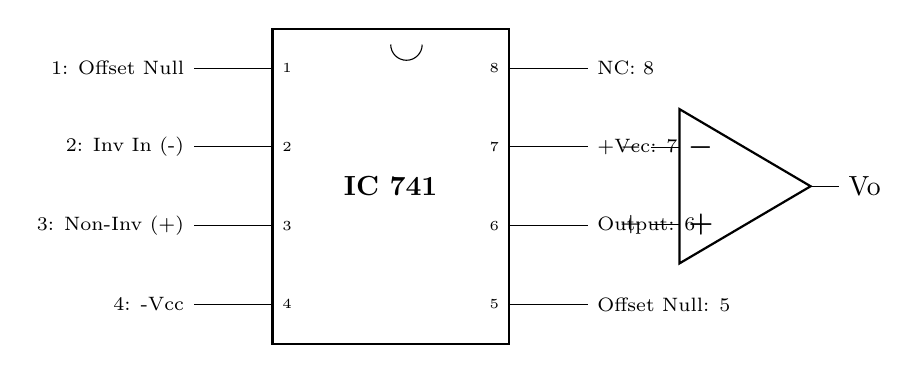
\begin{tikzpicture}
            % Pin Diagram
            \draw[thick] (0,0) rectangle (3,4);
            \node at (1.5, 2) {\textbf{IC 741}};
            \draw (1.5, 3.8) arc (180:360:0.2); % Notch
            
            % Pins
            \foreach \y/\p/\l in {3.5/1/Offset Null, 2.5/2/Inv In (-), 1.5/3/Non-Inv (+), 0.5/4/-Vcc} {
                \draw (0,\y) -- (-1,\y) node[left, font=\scriptsize]{\p: \l};
                \draw (0,\y) node[right, font=\tiny]{\p};
            }
            \foreach \y/\p/\l in {0.5/5/Offset Null, 1.5/6/Output, 2.5/7/+Vcc, 3.5/8/NC} {
                \draw (3,\y) -- (4,\y) node[right, font=\scriptsize]{\l: \p};
                \draw (3,\y) node[left, font=\tiny]{\p};
            }
            
            % Symbol
            \draw (6, 2) node[op amp] (op) {};
            \node at (op.+) [left] {$+$};
            \node at (op.-) [left] {$-$};
            % \node at (op.up) [above] {+V};
            % \node at (op.down) [below] {-V};
            \node at (op.out) [right] {Vo};
        \end{tikzpicture}
        \caption{IC 741 Pinout and Symbol}
    \end{figure}

    \textbf{Pin Description:}
    \begin{itemize}
        \item \textbf{2, 3}: Inputs (Inverting, Non-inverting).
        \item \textbf{6}: Output.
        \item \textbf{7, 4}: Power Supply ($+V_{CC}, -V_{EE}$).
        \item \textbf{1, 5}: Offset Null (to remove error voltage).
        \item \textbf{8}: No Connection.
    \end{itemize}
\end{solutionbox}

% Question 4(b)
\questionmarks{4(b)}{4}{Explain differential Amplifier using OPAMP.}
\begin{solutionbox}
    \textbf{Differential Amplifier:}
    Amplifies the difference between two input voltages.

    \begin{figure}[H]
        \centering
        \begin{circuitikz}[scale=0.8]
            \draw (0,0) node[op amp](op){};
            \draw (op.-) -- (-1, 0.5) to[R, l=$R_1$] (-3, 0.5) node[left]{$V_1$};
            \draw (op.+) -- (-1, -0.5) to[R, l=$R_1$] (-3, -0.5) node[left]{$V_2$};
            \draw (-1, -0.5) to[R, l=$R_2$] (-1, -2) node[ground]{};
            \draw (-1, 0.5) to[short] (-1, 1.5) to[R, l=$R_2$] (1, 1.5) -| (op.out);
            \draw (op.out) -- (2,0) node[right]{$V_{out}$};
        \end{circuitikz}
        \caption{Difference Amplifier}
    \end{figure}

    \textbf{Working:}
    Output $V_{out} = \frac{R_2}{R_1}(V_2 - V_1)$.
    Rejects common mode signals (CMRR).
    
    \begin{mnemonicbox}
        \mnemonic{CARE: Common-mode rejection, Amplifies difference, Resistor matching}
    \end{mnemonicbox}
\end{solutionbox}

% Question 4(c)
\questionmarks{4(c)}{7}{Explain the following parameters of an OP-Amp: 1)Input offset voltage 2) Output Offset Voltage 3) Input Offset Current 4)Input Bias Current 5) CMRR 6) Slew rate 7) Gain.}
\begin{solutionbox}
    \begin{itemize}
        \item \textbf{Input Offset Voltage ($V_{io}$):} Voltage applied at input to make output zero. (Typ: 1-5mV).
        \item \textbf{Output Offset Voltage:} Error voltage at output when inputs are zero.
        \item \textbf{Input Offset Current ($I_{io}$):} Difference between input bias currents $|I_{b1} - I_{b2}|$. (Typ: 10nA).
        \item \textbf{Input Bias Current ($I_{b}$):} Average of input currents $(I_{b1} + I_{b2})/2$. required to bias transistors.
        \item \textbf{CMRR:} Common Mode Rejection Ratio. $\text{CMRR} = A_d / A_{cm}$. Ability to reject noise. (Typ: 90dB).
        \item \textbf{Slew Rate (SR):} Max rate of change of output voltage. $SR = dV_o / dt|_{max}$. Unit: V/$\mu$s. (Typ: 0.5V/$\mu$s).
        \item \textbf{Gain ($A_{OL}$):} Open Loop Voltage Gain. ratio of output to differential input. (Typ: $2 \times 10^5$).
    \end{itemize}

    \begin{mnemonicbox}
        \mnemonic{VICS BGR: Voltage offset, Current offset, Slew rate, Bias, Gain, Rejection}
    \end{mnemonicbox}
\end{solutionbox}

% Question 4(a) OR
\questionmarks{4(a) OR}{3}{List characteristics of ideal op-amp.}
\begin{solutionbox}
    \begin{tabulary}{\linewidth}{|L|L|}
        \hline
        \textbf{Characteristic} & \textbf{Ideal Value} \\
        \hline
        Open Loop Gain ($A_{OL}$) & Infinite ($\infty$) \\
        \hline
        Input Impedance ($Z_{in}$) & Infinite ($\infty$) \\
        \hline
        Output Impedance ($Z_{out}$) & Zero ($0$) \\
        \hline
        Bandwidth (BW) & Infinite \\
        \hline
        CMRR & Infinite \\
        \hline
        Slew Rate & Infinite \\
        \hline
        Offset Voltage & Zero \\
        \hline
    \end{tabulary}

    \begin{mnemonicbox}
        \mnemonic{ZINC BOSS: Zero output Z, Infinite Gain/Input Z, No noise, CMRR infinite}
    \end{mnemonicbox}
\end{solutionbox}

% Question 4(b) OR
\questionmarks{4(b) OR}{4}{Draw and explain the block diagram of the Operational Amplifier (OPAMP) in detail.}
\begin{solutionbox}
    \textbf{Block Diagram:}
    \begin{figure}[H]
        \centering
        \begin{tikzpicture}[gtu flow, node distance=1.5cm]
            \node (In) [gtu block] {Input Stage\\(Diff Amp)};
            \node (Int) [gtu block, right=of In] {High Gain\\Stage};
            \node (Level) [gtu block, right=of Int] {Level\\Shifter};
            \node (Out) [gtu block, right=of Level] {Output\\Stage};
            
            \draw [gtu arrow] (In) -- (Int);
            \draw [gtu arrow] (Int) -- (Level);
            \draw [gtu arrow] (Level) -- (Out);
            \draw [gtu arrow] (Out) -- ++(1.5,0) node[right]{$V_{out}$};
            \draw [gtu arrow] (In) -- ++(-1.5,0) node[left]{Inputs};
            \draw [gtu arrow] (Level.south) -- ++(0,-1) node[below] {Feedback/Comp};
        \end{tikzpicture}
        \caption{Op-Amp Internal Block Diagram}
    \end{figure}

    \textbf{Stages:}
    \begin{enumerate}
        \item \textbf{Input Stage:} Differential amplifier (Dual Input Balanced Output). High $Z_{in}$.
        \item \textbf{Intermediate Stage:} High gain voltage amplifier (Darlington pair).
        \item \textbf{Level Shifter:} Emitter follower to shift DC level to 0V.
        \item \textbf{Output Stage:} Push-pull amplifier for low $Z_{out}$ and current drive.
    \end{enumerate}
\end{solutionbox}

% Question 4(c) OR
\questionmarks{4(c) OR}{7}{Draw & explain Inverting and Non-inverting Op-amp amplifier with the derivation of voltage gain.}
\begin{solutionbox}
    \textbf{1. Inverting Amplifier:}
    \begin{figure}[H]
        \centering
        \begin{circuitikz}[scale=0.7]
            \draw (0,0) node[op amp](op){};
            \draw (op.+) -- (-1, -0.5) node[ground]{};
            \draw (op.-) -- (-1, 0.5) to[R, l=$R_1$] (-3, 0.5) node[left]{$V_{in}$};
            \draw (-1, 0.5) -- (-1, 1.5) to[R, l=$R_f$] (1, 1.5) -| (op.out);
            \draw (op.out) -- (2,0) node[right]{$V_{out}$};
        \end{circuitikz}
    \end{figure}
    \textbf{Gain:} Virtual ground at (-) input. Current $I = V_{in}/R_1$. Flows to $R_f$.
    $V_{out} = -I R_f = -(V_{in}/R_1)R_f$.
    $$A_v = -R_f/R_1$$

    \textbf{2. Non-Inverting Amplifier:}
    \begin{figure}[H]
        \centering
        \begin{circuitikz}[scale=0.7]
            \draw (0,0) node[op amp](op){};
            \draw (op.+) -- (-1, -0.5) -- (-2, -0.5) node[left]{$V_{in}$};
            \draw (op.-) -- (-1, 0.5) to[R, l=$R_1$] (-1, -1.5) node[ground]{};
            \draw (-1, 0.5) -- (-1, 1.5) to[R, l=$R_f$] (1, 1.5) -| (op.out);
            \draw (op.out) -- (2,0) node[right]{$V_{out}$};
        \end{circuitikz}
    \end{figure}
    \textbf{Gain:} Voltage divider feedback $V_- = V_{out} \frac{R_1}{R_1+R_f}$.
    Virtual short $V_- = V_+ = V_{in}$.
    $V_{in} = V_{out} \frac{R_1}{R_1+R_f}$.
    $$A_v = 1 + R_f/R_1$$

    \begin{mnemonicbox}
        \mnemonic{PING-PONG: Phase Inverted Negative Gain vs Positive Output Non-inverted Gain}
    \end{mnemonicbox}
\end{solutionbox}

% Question 5(a)
\questionmarks{5(a)}{3}{Draw and explain integrator using Op-Amp.}
\begin{solutionbox}
    \textbf{Integrator:}
    \begin{figure}[H]
        \centering
        \begin{circuitikz}[scale=0.8]
            \draw (0,0) node[op amp](op){};
            \draw (op.+) node[ground]{};
            \draw (op.-) -- (-1, 0.5) to[R, l=$R$] (-3, 0.5) node[left]{$V_{in}$};
            \draw (-1, 0.5) -- (-1, 1.5) to[C, l=$C$] (1, 1.5) -| (op.out);
            \draw (op.out) -- (2,0) node[right]{$V_{out}$};
        \end{circuitikz}
        \caption{Ideal Integrator}
    \end{figure}
    \textbf{Working:} Output is proportional to time integral of input.
    $V_{out} = -\frac{1}{RC} \int V_{in} dt$.
    Used in analog computers and wave shaping.

    \begin{mnemonicbox}
        \mnemonic{TIME: Takes Input and Makes integral over time}
    \end{mnemonicbox}
\end{solutionbox}

% Question 5(b)
\questionmarks{5(b)}{4}{Compare different types of power amplifier.}
\begin{solutionbox}
    \begin{tabulary}{\linewidth}{|l|c|c|c|c|}
        \hline
        Parameter & Class A & Class B & Class AB & Class C \\
        \hline
        Conduction & $360^\circ$ & $180^\circ$ & $180^\circ-360^\circ$ & $<180^\circ$ \\
        \hline
        Efficiency & 25-50\% & 78.5\% & 50-70\% & >80\% \\
        \hline
        Distortion & Low & High & Low & High \\
        \hline
        Usage & Audio & General & Audio & RF \\
        \hline
    \end{tabulary}
    \begin{mnemonicbox}
        \mnemonic{CABINET: Conduction, Amplification, Biasing, Ideal apps, Noise, Efficiency, Temperature}
    \end{mnemonicbox}
\end{solutionbox}

% Question 5(c)
\questionmarks{5(c)}{7}{List applications of IC555 and explain any one in detail.}
\begin{solutionbox}
    \textbf{Applications:} Timers, Oscillators, Pulse generation, PWM, Frequency divider, Tone generator.

    \textbf{Astable Multivibrator:}
    \begin{figure}[H]
        \centering
        \begin{circuitikz}[scale=0.7]
            \draw (0,0) rectangle (3,4);
            \node at (1.5,2) {555};
            \draw (0,3.5) -- (-1,3.5) -- (-1,4.5) to[R, l=$R_1$] (-1,6) node[vcc]{$V_{CC}$};
            \draw (-1,3.5) to[R, l=$R_2$] (-1,1.5) -- (0,1.5); % Pin 6/2 area
            \draw (-1,1.5) to[C, l=$C_1$] (-1,0) node[ground]{};
            \draw (0,0.5) -- (-2,0.5) node[ground]{}; % Pin 1
            \draw (3,3.5) -- (4,3.5) node[vcc]{$V_{CC}$}; % Pin 8
            \draw (3,2) -- (4,2) node[right]{Output}; % Pin 3
            % Connections
            \draw (0,2.5) -- (-0.5,2.5) -- (-0.5, 3.5); % Pin 7 to R1-R2 junction
            \draw (-0.5, 3.5) -- (-1, 3.5);
            \draw (0, 1) -- (-1, 1) -- (-1, 1.5); % Pin 2 to C
            \draw (0, 3) -- (-0.5, 3) -- (-0.5, 1); % Pin 6 to C (Threshold)
        \end{circuitikz}
        \caption{Astable Mode}
    \end{figure}

    \textbf{Working:}
    Capacitor C charges through $R_1+R_2$ and discharges through $R_2$.
    $t_{high} = 0.693(R_1+R_2)C$.
    $t_{low} = 0.693 R_2 C$.
    $f = \frac{1.44}{(R_1+2R_2)C}$.
    Produces square wave output.
\end{solutionbox}

% Question 5(a) OR
\questionmarks{5(a) OR}{3}{Draw and explain summing amplifier using Op-Amp.}
\begin{solutionbox}
    \textbf{Summing Amplifier:}
    \begin{figure}[H]
        \centering
        \begin{circuitikz}[scale=0.7]
            \draw (0,0) node[op amp](op){};
            \draw (op.+) node[ground]{};
            \draw (op.-) -- (-1, 0.5) -- (-1, 1.5) to[R, l=$R_f$] (1, 1.5) -| (op.out);
            \draw (-1, 0.5) -- (-2, 0.5);
            \draw (-2, 0.5) to[R, l=$R_1$] (-4, 0.5) node[left]{$V_1$};
            \draw (-2, 0.5) -- (-2, -0.5) to[R, l=$R_2$] (-4, -0.5) node[left]{$V_2$};
            \draw (-2, -0.5) -- (-2, -1.5) to[R, l=$R_3$] (-4, -1.5) node[left]{$V_3$};
            \draw (op.out) -- (2,0) node[right]{$V_{out}$};
        \end{circuitikz}
    \end{figure}
    \textbf{Working:} $V_{out} = -(\frac{R_f}{R_1}V_1 + \frac{R_f}{R_2}V_2 + \dots)$.
    If all R equal, $V_{out} = -(V_1+V_2+V_3)$.
\end{solutionbox}

% Question 5(b) OR
\questionmarks{5(b) OR}{4}{Compare between push-pull amplifier and Complementary push-pull power amplifier.}
\begin{solutionbox}
    \begin{tabulary}{\linewidth}{|l|L|L|}
        \hline
        Feature & Push-Pull & Complementary Push-Pull \\
        \hline
        Transistors & Same type (NPN) & Matches Pair (NPN+PNP) \\
        \hline
        Transformers & 2 Required (Input/Output) & None \\
        \hline
        Size/Weight & Bulky & Compact \\
        \hline
        Cost & High & Low \\
        \hline
        Matching & Transistors only & NPN and PNP characteristics \\
        \hline
    \end{tabulary}
    \begin{mnemonicbox}
        \mnemonic{TONIC: Transformers, One type vs Complementary, Nice frequency, Improved distortion, Cost}
    \end{mnemonicbox}
\end{solutionbox}

% Question 5(c) OR
\questionmarks{5(c) OR}{7}{Draw pin diagram and block diagram of IC555 and explain in detail.}
\begin{solutionbox}
    \textbf{IC 555 Block Diagram:}
    \begin{figure}[H]
        \centering
        \begin{tikzpicture}[gtu flow]
            \node (Vcc) [coordinate] at (0,4) {};
            \node (Gnd) [coordinate] at (0,-4) {};
            \node (Div1) [gtu block, align=center] at (0, 2) {Comparator 1\\(Threshold)};
            \node (Div2) [gtu block, align=center] at (0, -2) {Comparator 2\\(Trigger)};
            \node (FF) [gtu block, right=of Div1] at (3,0) {Flip-Flop\\(RS)};
            \node (Out) [gtu block, right=of FF] {Output\\Stage};
            \node (Dis) [gtu block, below=of FF] {Discharge\\Transistor};
            
            \draw [gtu arrow] (Div1) -- (FF);
            \draw [gtu arrow] (Div2) -- (FF);
            \draw [gtu arrow] (FF) -- (Out);
            \draw [gtu arrow] (FF) -- (Dis);
            
            % Pins
            \draw (Div1.west) -- ++(-1,0) node[left]{6 (Thresh)};
            \draw (Div2.west) -- ++(-1,0) node[left]{2 (Trig)};
            \draw (Out.east) -- ++(1,0) node[right]{3 (Out)};
            \draw (Dis.south) -- ++(0,-0.5) node[below]{7 (Disch)};
            \draw (FF.north) -- ++(0,1) node[above]{4 (Reset)};
        \end{tikzpicture}
        \caption{Internal Block Diagram of IC 555}
    \end{figure}
    \textbf{Components:}
    \begin{enumerate}
        \item \textbf{Resistor Divider:} Three 5k$\Omega$ resistors set reference voltages ($2/3 V_{CC}, 1/3 V_{CC}$).
        \item \textbf{Comparators:} Compare inputs with references.
        \item \textbf{Flip-Flop:} Set/Reset by comparators.
        \item \textbf{Output Stage:} High current totem-pole output.
        \item \textbf{Discharge Transistor:} Discharges timing capacitor.
    \end{enumerate}

    \begin{mnemonicbox}
        \mnemonic{VICTOR: Voltage divider, Internal comparators, Control flip-flop, Timing, Output, Reset}
    \end{mnemonicbox}
\end{solutionbox}

\end{document}
